%\svnkwsave{$RepoFile: siminos/chao/exerFlow.tex $}
%\svnidlong {$HeadURL$}
%{$LastChangedDate$}
%{$LastChangedRevision$} {$LastChangedBy$}
%\svnid{$Id$}


\chapter{Exercises}
\label{sect:exerFlow}

\exercise{Birkhoff coordinates.}{\label{ex_birkhoff}
\index{Birkhoff!coordinates}
                                            \toCB
\PCedit{[Predrag 18apr2011 - not edited yet]}
In a plane billiard the ball travels between bounces
 along a straight line with a constant velocity--so the
4\dmn\ phase space flow can be reduced to a 2\dmn\ map
$\PoincM_{\Ssym{k} \leftarrow \Ssym{j}}$ that maps the
coordinates (Poincar\'e section $\PoincS_k$)
of the pinball from one disk edge to another.

A billiard flow has a natural Poincar\'e section
defined by Birkhoff coordinates $\arc_n$,
the arc length position of the $n$th bounce measured
along the billiard boundary,  % (\reffig{f-3disk}\,(b)),
and $\mompar_n= |p| \sin \phi_n$, the
momentum component parallel to the boundary, where $\phi_n$ is
the angle between the outgoing trajectory and the normal to the boundary.
We measure both the arc length $\arc$,
and the parallel momentum $\mompar$
counterclockwise relative to the outward normal%
. %(see \reffig{f-pinbAngles} as well as \reffig{FigIntroThreeA}).
In $\DOF=2$, the Poincar\'e section is a cylinder (topologically
an annulus),
% \reffig{f:BirkhoffCyl},
where the parallel momentum $\mompar$ ranges
for $-|p|$ to  $|p|$, and the $\arc$ coordinate is cyclic
along each connected component of $\partial Q$.
%\PC{label the two areas $Q_1$, $Q_2$ in \reffig{f:BirkhoffCyl}.
%Draw corresponding rectangles?}
The volume in the full phase space is preserved by the
Liouville theorem%
. % \refeq{LiuvVolCons}.
% The
Prove that the Birkhoff coordinates $x=(\arc,\mompar) \in \PoincS$,
% see \reffig{f-pinbAngles},
are the natural choice,
because with them the Poincar\'e return map
preserves the phase space volume of the $(\arc,\mompar)$ parameterized
Poincar\'e section
(a perfectly good coordinate set $(\arc, \phi)$ does not do that).
\index{Birkhoff!coordinates}
%\exerbox{ex_birkhoff}
% and they are easy to extract from the pinball trajectory.
% \toSect{c_buni_curv}

Without loss of generality we set $m=|v|=|p|=1$. % throughout.
Poincar\'e section condition eliminates one dimension, and the
energy conservation
$|p|=1$ eliminates
another, so the Poincar\'e section return map \PoincM\ is
$(2\DOF-2)$-dimensional.


Just after
the moment of impact the trajectory  is defined by $\arc_n$, the arc-length
position of the $n$th bounce along the billiard wall, and
$\mompar_n= p \sin \phi_n$
the momentum component parallel to the billiard wall
at the point of impact,
\reffig{FigIntroThreeA}.

Prove that these coordinates (due to Birkhoff)
are phase space volume
preserving.

No need to reinvent the wheel;
use the same notation as ChaosBook, \ie, $\arc$ instead
$R \theta$.
%
%%%%%%%%%%%%%%%%%%%%%%%%%%%%%%%%%%%%%%%%%%%%%%%%%%%%%%%%%%%%%%%%%%
\SFIG{IntroThree1} {}{ Poincar\'e section coordinates for the
3-disk game of pinball.
    }{FigIntroThreeA}
%%%%%%%%%%%%%%%%%%%%%%%%%%%%%%%%%%%%%%%%%%%%%%%%%%%%%%%%%%%%%%%%%%

}

\begin{figure}
\centering
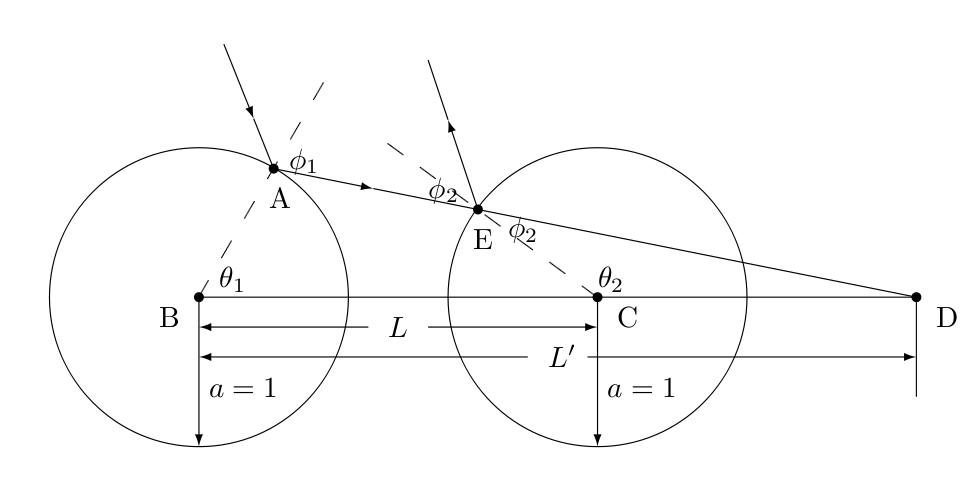
\includegraphics[width=\textwidth]{exr2-1}
\end{figure}


\solution{ex_birkhoff}{Birkhoff coordinates.}{

Assume the radius of two circles is $a=1$, the distance between the centers of two circles is L, the magnitude of the ball's momentum is 1. Thus, $p\sin{\phi} = \sin{\phi}$. Since the radius is 1, the arc-length is mumerically equal to the angle $\theta$ in the picture. Here we use the arclength s, which is equal to a$\theta$.

First, we have to find the map:$(s_{1},\sin(\phi_{1}))\mapsto(s_{2},\sin(\phi_{2}))$

Look at ${\Delta}ABD$, by Sine Theorem, we have $\frac{\sin({\pi}-\phi_{i})}{\overline{BD}} = \frac{\sin(\beta)}{\overline{AB}}$, where $\overline{BD} = L^{'}$, $\overline{AB} = a$, $\sin(\pi-\phi_{1}) = \sin(\phi_{1})$

\beq\Rightarrow \frac{\sin(\phi_{1})}{L^{'}} = \frac{\sin(\beta)}{R}\eeq

Look at ${\Delta}ECD$, still by Sine Theorem, we have $\frac{\sin(\beta)}{\overline{EC}} = \frac{\sin(\phi_{2})}{\overline{CD}}$, where $\overline{EC} = a$, $\overline{CD} = L^{'}-L$

\beq\Rightarrow \frac{\sin(\phi_{2})}{L_{'}-L} = \frac{\sin(\beta)}{a}\eeq

\beq\beta = \phi_{1}-\frac{s_{1}}{a}\eeq

From the first equation, we have
\beq L_{'} = \frac{\sin(\phi_{1})}{\sin(\beta)}a = \frac{\sin(\phi_{1})}{\sin(\phi_{1}-s_{1})}\eeq

Substitute this into the second equation, we have \beq\displaystyle\frac{\sin(\phi_{2})}{\frac{\sin(\phi_{1})}{\sin(\phi_{1}-\frac{s_{1}}{a})}a-L} = \frac{\sin(\phi_{1}-\frac{s_{1}}{a})}{a}\eeq
\beq\Rightarrow \sin(\phi_{2}) = \sin(\phi_{1})-\frac{L}{a}\sin(\phi_{1}-\frac{s_{1}}{a}) \eeq

Also we have $\frac{s_{2}}{a} = \pi-\phi_{2}-\beta = \pi-\phi_{2}-(\phi_{1}-\frac{s_{1}}{a})$

Now we have got the map. Next step is to show it's phase space volume preserving.

rewrite the map by substituting $p_{i} = \sin(\phi_{i}),\phi_{i} = \arcsin(p_{i})$:
\beq p_{2} = p_{1}-\frac{L}{a}p_{1}\cos(\frac{s_{1}}{a})+\frac{L}{a}\sqrt{1-p_{1}^{2}}\sin(\frac{s_{1}}{a}) \eeq
\beq \frac{s_{2}}{a} = \pi+\frac{s_{1}}{a}-\arcsin(p_{1})-\arcsin(p_{2}) \eeq

\begin{eqnarray}
dp_{2}&=&dp_{1}-\frac{L}{R}\cos(\frac{s_{1}}{a})dp_{1}+\frac{L}{a}\sin(\frac{s_{1}}{a})p_{1}d\frac{s_{1}}{a}-
\frac{Lp_{1}\sin(\frac{s_{1}}{a})}{a\sqrt{1-p_{1}^{2}}}dp_{1}+
\\\nonumber&&\frac{L}{a}\sqrt{1-p_{1}^{2}}\cos{\frac{s_{1}}{a}}d\frac{s_{1}}{a}\\\nonumber
&=&(1-\frac{L}{a}\cos{\frac{s_{1}}{a}}-\frac{Lp_{1}\sin(\frac{s_{1}}{a})}{a\sqrt{1-p_{1}^{2}}})dp_{1}
+(\frac{L}{a}\sin(\frac{s_{1}}{a})p_{1}+\frac{L}{a}\sqrt{1-p_{1}^{2}}\cos{\frac{s_{1}}{a}})d\frac{s_{1}}{a}\\\nonumber
d\frac{s_{2}}{a}&=&d\frac{s_{1}}{a}-\frac{1}{\sqrt{1-p_{1}^{2}}}dp_{1}-\frac{1}{\sqrt{1-p_{2}^{2}}}dp_{2}\\\nonumber
dp_{2}\wedge d\frac{s_{2}}{a}&=& (1-\frac{L}{a}\cos(\frac{s_{1}}{a})-\frac{Lp_{1}\sin(\frac{s_{1}}{a})}{a\sqrt{1-p_{1}^{2}}})dp_{1}{\wedge}d\frac{s_{1}}{a}+\\&&\frac{1}{\sqrt{1-p_{1}^{2}}}(\frac{L}{a}\sin(\frac{s_{1}}{a})p_{1}
+\frac{L}{a}\sqrt{1-p_{1}^{2}\cos(\theta_{1})})dp_{1}\wedge d\frac{s_{1}}{a}\\\nonumber
&=&dp_{1}\wedge d\frac{s_{1}}{a}\\
&&\Rightarrow dp_{2}\wedge ds_{2} = dp_{1}\wedge ds_{1}
\end{eqnarray}

Now let's look at map for $\frac{s}{a}$. We can rewrite it as:
\\ \beq \frac{s_{2}}{a} - \frac{s_{1}}{a} = \pi-\arcsin(p_{1})-\arcsin(p_{2}) \eeq
On the left hand side, $\frac{s_{2}}{a} - \frac{s_{1}}{a} = \theta_{2}-\theta_{1}$ is independent of the choice of coordinate. Any choice of start line of angle $\theta$ just varies up to a constant for both $\theta_{2}$ and $\theta_{1}$, so won't affect the validity of the demonstration.

Furthermore, we can take the radii of two circles unequal,
$a_{1} \neq a_{2}$. Definition of parallel momentum remain the same.
Thus we have $\theta_{1}=\frac{s_1}{a_1}$, $\theta_{2}=\frac{s_2}{a_2}$.
Follow the same route above to obtain the map:
\bea
p_{2} &=& p_{1}-Lp_{1}\cos(\frac{s_1}{a_1})+L\sqrt{1-p_1^2}\sin(\frac{s_1}{a_1})\\
s_{2} &=& \frac{a_2}{a_1}+{\pi}a_{2}-a_{2}\arcsin(p_1)-a_{2}\arcsin(p_2)
\eea
By writing out the full derivative of $dp_2$ and $ds_2$ in terms of
$dp_1$ and $ds_1$, we can obtain the Jacobian matrix
\bea
\left(
\begin{array}{c}
dp_2\\
ds_2
\end{array}
\right)
=
J
\left(
\begin{array}{c}
dp_1\\
ds_1
\end{array}
\right)\\
J = \\
\left(
\begin{array}{cc}
1-L\cos(\frac{s_1}{a_1})-\frac{Lp_1}{\sqrt{1-p_1^2}}\sin(\frac{s_1}{a_1})  &
\frac{L}{a_1}(p_1\sin(\frac{s_1}{a_1})+\sqrt{1-p_1^2}\cos(\frac{s_1}{a_1}))\\
-\frac{a_2}{\sqrt{1-p_1^2}}-(1-L\cos(\frac{s_1}{a_1})-\frac{Lp_1}{\sqrt{1-p_1^2}}\sin(\frac{s_1}{a_1})) &
\frac{a_2}{a_1}-\frac{L}{a_1}(p_1\sin(\frac{s_1}{a_1})+\sqrt{1-p_1^2}\cos(\frac{s_1}{a_1}))
\end{array}
\right)
\nonumber
\,.
\eea
This yields $|J|=\frac{a_2}{a_1}$, the ratio of radius of two
circles. When $a_2 = a_1$, the determinant of the Jacobian is 1, which
coincides with the previous result. Something is deeply wrong here.
    }%end  \solution{ex_birkhoff}{Birkhoff coordinates.
